%
% Kapitel: Usability
% Abschlussarbeit (Bachelor)
%
% Thema: Erstellung einer Browser Extension zur Usability Evaluierung von beliebigen Web-Applikationen über Heatmaps.
% Betreuer 1: Prof. Dr. Targo Pavlista
% Betreuer 2: Siamak Haschemi
%
% @author Christian Bromann <contact@christian-bromann.com>
%

\chapter{Usability}

Mit dem Substantiv \textit{Gebrauchstauglichkeit} übersetzt die ISO Norm 9241 den Begriff Usability und bezeichnet damit den Prozess der \glqq Benutzer-orientierte Gestaltung interaktiver Systeme\grqq{} \cite{iso9241}. Oft gleichgesetzt mit dem Fachgebiet der Human-Computer-Interaktion, beschreibt es das Bestreben dem Benutzer einer Software zu helfen, ein gewisses Ziel möglichst schnell und effizient zu erreichen. Es ist damit der wichtigste Erfolgsfaktor der Systemqualität. Die Bedienung des Computers ist dabei immer mit einer Aufgabe verbunden, die der Nutzer mithilfe einer Software versucht zu lösen. Dieses Prinzip lässt sich vereinfacht in ein Mensch-Maschinen-System zerlegen. Es basiert auf vier prinzipiellen Komponenten, die möglichst ergonomisch miteinander agieren sollen.

\vspace{0.6cm}
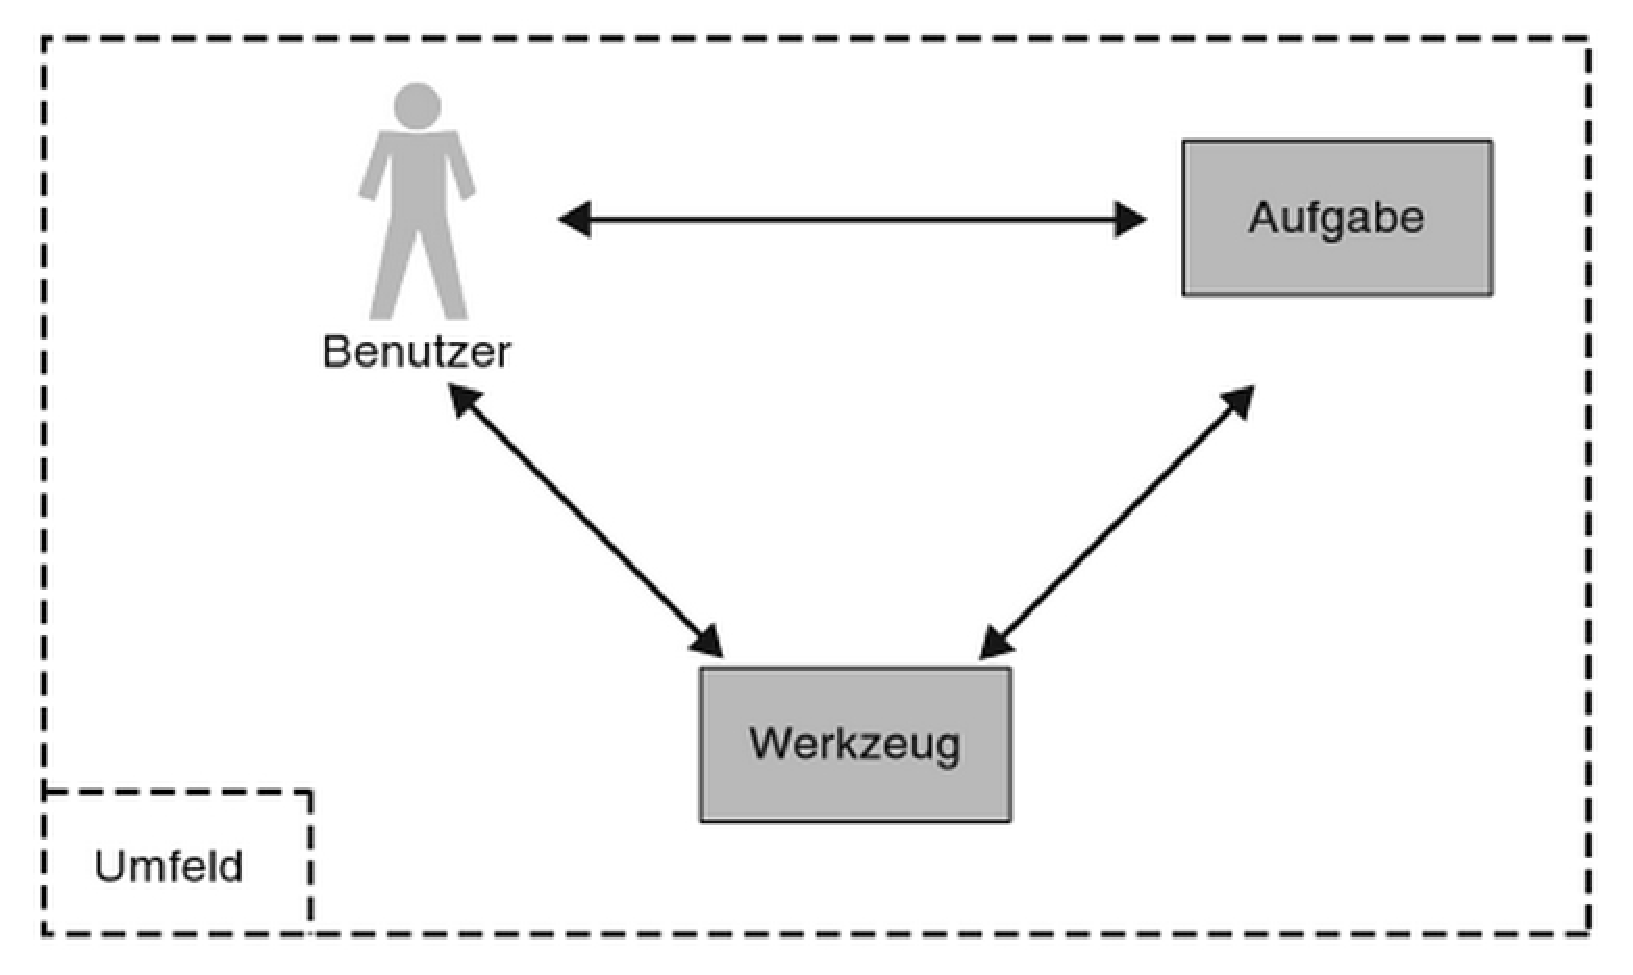
\includegraphics[scale=0.5]{./images/human-machine-system}
\begin{figure}[htb]
   \centering
   \caption{Mensch-Maschinen-System \textbf{Quelle:} \cite{UsabilityKompakt}}
    \label{mms}
\end{figure}

Die Eigenschaften und Funktionen einer Software bestimmen dabei nicht ausschließlich dessen Usability. So spielt das Einsatzumfeld ebenfalls eine wichtige Rolle. Beispielhaft ausgedrückt kann ein Flaschenöffner noch so handlich sein, wenn er dafür genutzt wird, Nägel in die Wand zu schlagen. Daher liegt eine benutzerfreundliche und ergonomische Software erst dann vor, wenn \glqq sie von den vorhergesehen Benutzern einfach erlernt und effizient verwendet werden [kann] und diese damit ihre beabsichtigen Ziele und Aufgaben zufriendenstellend [ausführt]\grqq{} \cite{UsabilityKompakt}.\\
\\
Um dies zu erreichen, sollte \textit{Usability Engineering} ein wichtiger Prozess in der Entwicklung einer Software sein. Angefangen von der Definition messbarer Usability Attribute über die Festlegung von numerischen Werten dieser bis hin zum Testen der Software ist dies ein sich immer wiederkehrendes Verfahren, bei dem sich die Methodik flexibel gestaltet. Die Attributen sollten möglichst einfache messbare Eigenschaften der Software darstellen und nach jedem Test mit den festgelegten Werten verglichen werden. Sind die Werte nicht erreicht worden, folgt eine Analyse der aufgetretenen Probleme und die anschließende Verbesserung der Software. Es handelt sich um einen iterativen Prozess, der nie wirklich einen Abschluss findet. Verbesserungen in der Usability sind immer möglich. Meist erreicht man jedoch einen zufriedenstellenden Grad der Benutzerfreundlichkeit oder hat keine Zeit oder Budget mehr für weitere Tests.\\
\\
\textit{Usability Testing} bezeichnet den gesamten Ablauf, bei dem überprüft wird, ob festgelegte Usability Ziele erreicht wurden oder nicht. Die Tests unterteilen sich in verschiedene Methoden, die unterschiedliche Daten für die heuristische Auswertung sammeln. Diese sollten in einer Vorbereitungsphase genau bestimmt werden und gewissen Kriterien unterliegen, damit sie ein genaues Abbild des Nutzerverhaltens widerspiegeln. Die Durchführung muss dabei nicht zwingend in einem Labor erfolgen. Oft verfälschen sogar Tests unter Laborbedingungen das Ergebnis, da der Benutzer der Software nicht in einem gewohntem Umfeld agiert und dadurch zu einem anderen Verhalten neigt. Eine festgeschrieben Mindestanzahl von Personen, die an dem Test teilnehmen, gibt es nicht. Nach Jakob Nielsen reichen schon 5 Probanden aus \cite{anzahlTestpersonen}, um einen großen Anteil der Probleme herauszufinden. Eine anschließende Analyse der Ergebnisse durch verschiedene Metriken deckt Schwachstellen in der Benutzung auf und kann mögliche Verbesserungen der Software herleiten.\\
\\
Im Laufe der letzten Jahrzehnte wurde für die Softwareentwicklung verschiedene Vorgehensmodelle entwickelt um eine koordinierte Vorgehensweise für die Erstellung von Software zu gewährleisten. Modelle, wie zbs. das Wasserfallmodell oder das V-Modell, werden in der Realität jedoch kaum wirklich eingehalten. Es enstehen immer wieder Mischformen, bei denen Elemente der benutzerorientierten Entwicklung integriert werden. Dieser, als sogenannte \textit{Usability Engineering Lifecycle} bezeichnete, Prozess bringt nach der Analyse- und Entwicklungsphase noch eine eine Nutzungsphase mit sich, da davon ausgegangen wird, dass \glqq trotz sorgfältiger Analyse und Entwicklung einige Nutzungsprobleme [sich] erst im Echtbetrieb herausstellen\grqq{} \cite{lifecycle}.

%
% Usability I'm Web
% Abschlussarbeit (Bachelor)
%
% Thema: Erstellung einer Browser Extension zur Usability Evaluierung von beliebigen Web-Applikationen über Heatmaps.
% Betreuer 1: Prof. Dr. Targo Pavlista
% Betreuer 2: Siamak Haschemi
%
% @author Christian Bromann <contact@christian-bromann.com>
%

\section{Usability im Web}

% Usability lässt sich nicht via Testscript Testen, sondern hängt immer ab von den verschiedenen Einflüsse der Benutzer
% http://usabilitygeek.com/an-introduction-to-website-usability-testing/
% http://usabilitygeek.com/wp-content/uploads/2011/06/International-Journal-of-Human-Computer-Interaction-IJHCI-Volume-2-Issue-1.pdf
%
% Einflüsse
% Abschlussarbeit (Bachelor)
%
% Thema: Erstellung einer Browser Extension zur Usability Evaluierung von beliebigen Web-Applikationen über Heatmaps.
% Betreuer 1: Prof. Dr. Targo Pavlista
% Betreuer 2: Siamak Haschemi
%
% @author Christian Bromann <contact@christian-bromann.com>
%

\section{Einflüsse}

% Was kann die Benutzbarkeit beeinflussen
% Barrierefreiheit
% X-Browser Gleichheit
%
% Metriken
% Abschlussarbeit (Bachelor)
%
% Thema: Erstellung einer Browser Extension zur Usability Evaluierung von beliebigen Web-Applikationen über Heatmaps.
% Betreuer 1: Prof. Dr. Targo Pavlista
% Betreuer 2: Siamak Haschemi
%
% @author Christian Bromann <contact@christian-bromann.com>
%

\section{Metriken und Analyse}

Usability ist keine Eigenschaft, die einfach und exakt abzulesen ist. Um sie herauszufinden, gibt es zwei Möglichkeiten. Entweder man vertraut seinen eigenem Gefühl beim Benutzen der Software oder erstellt Tests und nutzte Metriken zur Auswertung der Ergebnisse. Die Intuition ist wichtig und kann viel aussagen, bietet jedoch keine Sicherheit, da sie lediglich die eigene Meinung repräsentiert. Da eine Software jedoch von verschiedenen Personen benutzt wird, die jeweils unterschiedliche Ansprüche an das Produkt stellen, reicht das eigene Gefühl nicht aus. Eine Usability Studie bringt ein allgemeineres Abbild der Benutzbarkeit. Die aus den Tests erzeugten Daten lassen sich durch verschiedenste Metriken analysieren und auswerten.\\
\\
Usability Tests unterliegen keinen Richtlinien. Sie sind sehr unterschiedlich und spezialisieren sich teilweise auf bestimmte Aspekte bei der Benutzung einer Software. Abhängig davon, welche Aspekte analysiert werden und welche Daten dabei aufgezeichnet werden, müssen Metriken ganze individuell für jeden Test erstellt werden. Sie bilden das Maß der Benutzbarkeit und sollten objektiv bestimmbar und vergleichbar sein.

\subsection{Clickmaps}
\subsection{Heatmaps}
\subsection{Gazespots}
\subsection{Gazeplots}
\subsection{Attention Maps}
%
% Marktanalyse
% Abschlussarbeit (Bachelor)
%
% Thema: Erstellung einer Browser Extension zur Usability Evaluierung von beliebigen Web-Applikationen über Heatmaps.
% Betreuer 1: Prof. Dr. Targo Pavlista
% Betreuer 2: Siamak Haschemi
%
% @author Christian Bromann <contact@christian-bromann.com>
%

\section{Marktanalyse}

Die Durchführung von Usability Tests geschieht vornehmlich in Laboren und ist meist mit hohen Kosten verbunden. Eine Online-Agentur oder ein Startup kann diese Kosten nicht aufbringen. Oft werden deshalb diese Tests gar nicht durchgeführt und bleiben lediglich für profitbringende Webseiten mit Werbung eine Option. Die einzige Möglichkeit, die Usability der eigenen Seite halbwegs genau zu testen, ist der Verzicht auf Labortests und die Nutzung von Onlinetools. Diese gibt es mittlerweile in verschiedensten Varianten. Nur wenige von ihnen sind kostenlos. In diesem Kapitel werden drei Tools von unterschiedlicher Funktionsbreite vorgestellt und vergleicht.

\subsection*{CrazyEgg\footnote{\url{http://www.crazyegg.com/}}}

Dieses sehr populäre Tool zeichnet alle Klicks der User einer Website auf und ist in der Lage die Daten in den verschiedenster Formen informativ zu visualisieren. Neben den gewöhnlichen Attention- und Clickmaps, bietet das Feature \textit{Confetti} die Möglichkeit, hinter jedem Klick die Herkunft des Besuchers festzustellen. Das Tool ist zudem in der Lage, jegliche Elemente auf der Seite, wie z. B. Links, Bilder oder Überschriften, zu erkennen und die Rate der Klicks dieser anzuzeigen. Eingebunden wird es durch das Einfügen eines JavaScript Codeschnippsels auf der eigenen Seite. Die Auswertung erfolgt auf der Toolseite und ist als Excel Datei exportierbar.

\subsubsection*{Vorteile}
Es bietet trotz des günstigen Preises eine Reihe von gebräuchlichen Visualisierungen, die dabei helfen können, die Usability der Seite zu steigern.

\subsubsection*{Nachteile}
Das Tool analysiert lediglich das Klick- und Scrollverhalten der User für eine individuelle Seite. Daraus lassen sich keine Schlüsse auf den Gesamtcontext des Besuches ziehen. Es ist dadurch schwer herauszufinden warum der User geklickt hat.

\subsubsection*{Preis}
Angeboten werden vier verschieden Pläne von 9\$ bis hin zu 99\$.

\subsection*{Loop$^{11}$ \footnote{http://www.loop11.com/}}

Loop$^{11}$ ist ein Task basiertes Usability-Testing-Tool. Die Tests werden von ausgewählten Probanden durchgeführt und müssen dabei nicht durch den Seitenbetreiber moderiert werden. Dieser muss lediglich einen Testcase mit verschiedenen Aufgaben erzeugen und ihn an ausgewählte User schicken. Die Probanden werden dann mit einer Aufgabe konfrontiert, entscheiden aber selbstständig, wann sie diese erfüllt haben oder nicht. In der Auswertung ist anschließend die Erfolgsrate und die dafür benötigte Zeit einsehbar. Zudem ist es möglich Besucherpfade zu analysieren. Das Tool benötigt dabei keine Software. Die getestete Seite wird in einem eigenen iFrame eingebunden und analysiert. Es ist dadurch möglich jede frei zugängliche Seite des Internets zu testen.

\subsubsection*{Vorteile}
Es muss kein Code implementiert werden, wodurch es möglich ist, jede beliebige Seite des Internets zu testen.

\subsubsection*{Nachteile}
Die Probanden können selbst entscheiden, wann die Aufgabe gelöst ist. Die Entscheidung des Users kann im Nachhinein nicht erfragt oder ausgewertet werden.

\subsubsection*{Preis}
Für die Nutzung des Tools werden Lizenzen für 158\$ bis hin zu 825\$ pro Monat verkauft.

\subsection*{Mouse Eye Tracking\texttrademark \footnote{http://met.picnet.com.au/}}

Das mit zwei \textit{iAwards} ausgezeichnete Tool \textit{Mouse Eye Tracking\texttrademark} bietet neben Click- und Heatmaps viele nützliche Visualisierungen vom Verhalten der User an. Es ist sogar möglich, die Mausposition eines einzigen Besuchers, über den kompletten Zeitraum des Aufenthaltes auf der Seite, zu verfolgen. Ebenfalls werden Besucherpfade gespeichert und analysiert. Eingebunden wird es standardgemäß mit dem Einfügen von JavaScript Code im HTML.

\subsubsection*{Vorteile}
Die Analyse des Nutzerverhaltens ist sehr granular. Es ist sogar möglich den Mausverlauf eines einzelnen Benutzers zu analysieren.

\subsubsection*{Nachteile}
Die Aufzeichnung der Daten erfolgt ohne jegliche Vorraussetzungen an den Benutzer, in Form von z.B. Tasks. Die Intention des Users für sein Verhalten ist dadurch schwer einschätzbar.

\subsubsection*{Preis}
Nach einer 7-tägigen Probephase kann der Kunde ein Paket für 10\$ oder 20\$ pro Monat wählen.
















%
% Mensch vs. Maschiene
% Abschlussarbeit (Bachelor)
%
% Thema: Erstellung einer Browser Extension zur Usability Evaluierung von beliebigen Web-Applikationen über Heatmaps.
% Betreuer 1: Prof. Dr. Targo Pavlista
% Betreuer 2: Siamak Haschemi
%
% @author Christian Bromann <contact@christian-bromann.com>
%

\section{Mensch vs. Maschine}

Zu Beginn dieses Kapitels wurde Usability als eine Art Bestreben nach ergonomischer Software definiert. In dem Mensch-Maschienen-System spielte dabei der User eine wichtige Schlüsselkomponente zum Erreichen dieses Vorhabens. Je nach Alter, Erfahrung und Intention nutzen Menschen eine Software sehr unterschiedlich. Dadurch scheint es, als ob immer eine Person zur Bestimmung der Usability involviert sein muss, um ein aussagekräftiges Resultat zu erzielen. Es stellt sich die Frage auf, ob dies wirklich so ist!\\
\\
Der Begriff \textit{Informatik} ist die Komposition aus den Wörtern Information und Automatik / Mathematik. Jeder Informatiker strebt danach für doppelt ausgeführte Handlungen einen Automatismus zu entwerfen, um sich unnötige Arbeit zu sparen. Dies soll jedoch nicht suggerieren, dass Informatiker faule Menschen sind \cite{lazy}. Beim Usability Engineering findet ebenfalls ein immer wieder auftretender Prozess der Analyse und Verbesserung statt. Dieser ist meist immer mit hohen Kosten und Zeitaufwand verbunden. Zudem führen Usability Tests aufgrund des sogenannten \textit{\glqq Evaluator Effect\grqq{}} \cite{anzahlTestpersonen} nicht immer zu den gewünschten Ergebnissen. Ein Grund dafür ist die kritische Rolle der Gutachter. Studien haben bewiesen, dass diese zu unterschiedlichen und teilweise falschen Interpretationen neigen und Probleme beweisen, die bereits entdeckt wurden.\\
\\
Nicht nur aufgrund dieser Tatsachen haben sich bereits viele Usabiliy Experten mit der Frage beschäftigt, wie die Benutzerfreundlichkeit auf Webseiten automatisiert getestet und in Ergebnisse überführt werden kann \cite{automatisierteUsabilityTests}. Daraus entstanden im Laufe der Zeit verschiedene Prototypen, die sich bereits auf dem Markt etablieren konnten. Diese nutzen entweder die bisher entwickelten Normen der Organisationen für Standardisierung oder versuchen ein mögliches Nutzerverhalten vorauszusehen. Letztere Herangehensweise wurde bereits von vielen Wissenschaftlern kritisiert, da die dafür verwendeten Algorithmen zum Vorhersagen des Verhaltens zu teilweise beirrenden Ergebnissen führen.\\
\\
Anders dagegen nutzt das Framework \textit{USEFul} ein Regelset, welches den verschiedenen Normen der Usability entspricht, zur Analyse der Seite und zur Einschätzung der Benutzerfreundlichkeit. Dieses Regelset wird dabei in drei verschiedene Kategorien untergliedert. Eine Kategorie entspricht den Richtlinien, die das Tool im vollem Umfang evaluieren und kontrollieren kann. Sie sind ablesbar und über Parameter klassifizierbar. Die nächste Kategorie beinhaltet Normen, die nur teilweise erfassbar und messbar sind. Zu abstrakte Usability Regeln fallen schließlich in die letzte Kategorie. Diese sollten von den Evaluatoren manuell kontrolliert werden, ob sie für die aktuell getestete Seite zutreffen oder nicht. Zusätzlich werden die Regeln von 1 bis 5 priorisiert, um wichtigen Guidelines eine höhere Gewichtung zu geben.\\
\\
Laut Nielsen ist die URL ein Teil des User Interfaces und bestimmt somit ebenfalls die Usability einer Website \cite{urlasui}. Sie sollte so kurz und prägnant wie nötig gehalten werden und sich an der Seitenstruktur orientieren. Diese nicht ganz unwichtige Regel ist ein gutes Beispiel, um aufzuzeigen wie USEFull eine Website automatisiert evaluieren kann. Nachdem sich das Tool die Source Dateien der Seite gezogen hat, sucht es nach allen Link Tags auf der Seite. Diese Tags beinhalten die Ziel URL im \textit{href} Attribut. Überschreitet die URL die Länge der vorher festgelegten maximalen Anzahl von Zeichen, so verstößt die Seite gegen diese Regel. Berechnet man nun das Verhältnis der korrekten gegenüber der zu langen URLs, so erhält man sogar eine Qualitätsrate, die zwischen verschiedenen Tests verglichen werden kann. Abbildung \ref{usefull} zeigt die letztendliche Gesamtauswertung des Frameworks. Die Ergebnisse werden innerhalb der jeweiligen Kategorien aufgelistet, nach Priorität sortiert und erklärt.

\vspace{0.3cm}
\begin{center}
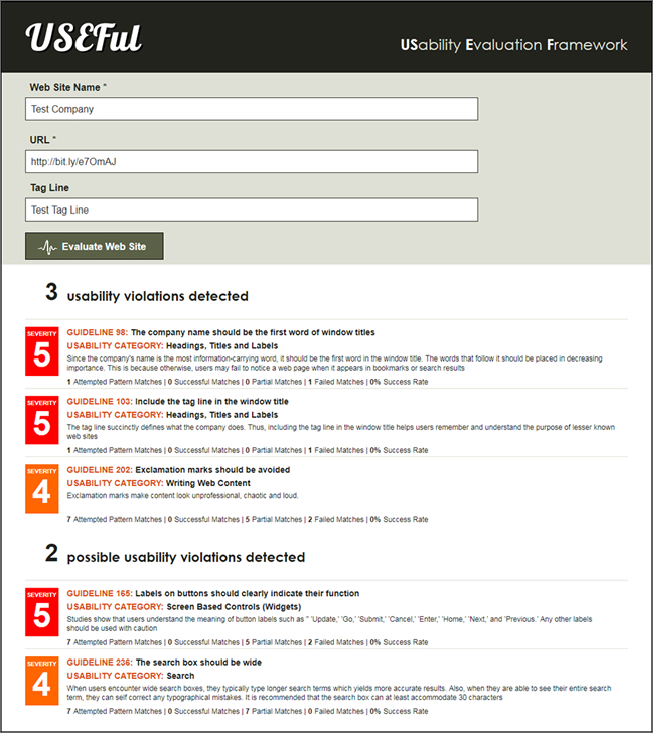
\includegraphics[scale=1]{./images/usefull}
\end{center}
\begin{figure}[htb]
   \centering
   \caption{Ansicht einer automatisierten Auswertung des USEFull Frameworks\\\textbf{Quelle:} http://usabilitygeek.com/wp-content/uploads/2012/03/USEFul-A-Framework-To-Automate-Website-Usability-Evaluation-Analysis.jpg}
    \label{usefull}
\end{figure}

Unglücklicherweise ist der Prototyp noch nicht für die Öffentlichkeit zugänglich. Lediglich Papers und Usability Blogs beschreiben die Funktionsweise und Features des Tools. Nichtsdestotrotz scheint der Traum nach einer komplett automatisierten Usability Evaluierung auch damit nicht erfüllt zu sein. Da nicht wirklich alle Regeln mit Algorithmen überprüft werden können, bleibt es letztendlich die Aufgabe eines Experten zu entscheiden, ob die Ergebnisse der Auswertung repräsentativ genug sind, um die Qualität der Usability richtig einzustufen. Dennoch können viele Aspekte automatisiert kontrolliert werden und dadurch bei der Entwicklung frühzeitig die Probleme aufdecken, die ohne das Tool erst durch teure Tests erkannt werden können.












